\documentclass{article}
\usepackage[utf8]{inputenc}
\usepackage{amsmath, amssymb, amsfonts}
\usepackage{geometry}
\usepackage{graphicx} % Required for inserting images
\usepackage{amsthm}
\geometry{a4paper, margin=1in}
\usepackage{parskip}
\setlength{\parindent}{0pt}
\usepackage{xcolor}
\pagecolor{black}
\color{white}
\usepackage{cancel}
\usepackage{tikz}
\newcommand{\Ric}{\mathcal{R}}

\newtheorem{theorem}{Theorem}[section]
\newtheorem{definition}{Definition}[section]
\newtheorem{prop}{Proposition}[section]
\newtheorem{ex}{example}[section]
\title{General Relativity}
\author{Frankie Yang, Genius Ivy}
\date{}


\begin{document}
\maketitle

\tableofcontents
\newpage
\section{Differential Geometry}

 \subsection{Connection and Covariant Derivative}
At each point $p$ of a manifold $M$ there is a tangent space $T_pM$ with corrdinate basis $\{\partial_\mu\}$. A vector is $V=V^\mu \partial_\mu$. Since $V$ itself does not depend on the chart and $\partial_\alpha = \frac{\partial x^\mu}{\partial x'^\alpha}\partial_\mu$. The component must transform as
\begin{equation}
    V'^\alpha = \frac{\partial x'^\alpha}{\partial x^\mu}V^\mu
\end{equation}

Differentiating $V$ is comparing the vector at two different point $V(p)\in T_pM $ and $V(p+dp) \in T_{p+dp}M$. These are in two different vector spaces, and a bare manifold gives no way to identify them. Thus, we need a connection to compare vectors at different points.
\begin{definition}
An affine connection assigns to vector fields $X,Y$ a vector field $\nabla _X Y$ such that
\begin{itemize}
    \item $\nabla_{fX+gY} Z= f\nabla_XZ + g\nabla_Y Z$. Its linear over functions in the direction slots.
    \item $\nabla_X(Y+Z) = \nabla_X Y + \nabla_X Z$
    \item $\nabla_X(fY) = X(f)Y + f\nabla_X Y$. Leibniz rule.
\end{itemize}
\end{definition}

In which $X(f) = X^\mu \partial_\mu f$, and on scalars we set $\nabla_X f = X(f)$. The connection is a bilinear map that takes two vector fields and produces another vector field, capturing the idea of how one vector field changes along the direction of another.

We have $\nabla _{\partial_\mu}\partial_\nu$ as a vector, so we can expand it in the basis $\{\partial_\mu\}$ as
\begin{equation}
    \nabla_{\partial_\mu}\partial_\nu \equiv \Gamma^\lambda_{~~\mu\nu} \partial_\lambda
\end{equation}

The first index gives the direction of differentiation. We can expand a general $\nabla_XY$ using the later 2 axioms:
\begin{equation}
    \nabla_XY=X^\mu\nabla_{\partial_\mu}\left(Y^\nu\partial_\nu\right)=X^\mu\left[\left(\partial\mu Y^\nu\right)+Y^\nu\Gamma^\lambda_{~~\mu\nu}\partial_\lambda\right]
\end{equation}

Then the components of the derivative is given by

\begin{equation}
    \boxed{\nabla_\mu Y^\lambda = \partial_\mu Y^\lambda +\Gamma^\lambda_{~~\mu\nu}Y^\nu},
\end{equation}
which is the form for \textbf{Covariant Derivative}.

Now, we can extend this to all tensors. We further demand two requirements: $\nabla$ obeys the Leiniz rule on tensor products, and it commutes with contractions. Applying this to the scalar $\omega_\nu Y\nu$:

\begin{equation}
    \partial_\mu(\omega_\nu Y^\nu) = \partial_\mu(\omega_\nu)Y^\nu + \omega_\nu(\partial_\mu Y^\nu + \Gamma^\nu_{~~\mu\lambda}Y^\lambda)\implies \nabla_\mu \omega_\lambda = \partial_\mu \omega_\lambda - \Gamma^\nu_{~~\mu\lambda}\omega_\nu
\end{equation}

As the derivative for the scalar must be $\partial_\mu \omega_\nu Y^\nu + \omega_\nu \partial_\mu Y^\nu$. Then we have the general rule: $+\Gamma$ for upper index and $-\Gamma$ for lower index.

\subsection{Transformation of $\Gamma$}

With the basis-vector definition $\nabla_{\partial'_\beta} \partial'_\gamma = \Gamma'^\alpha_{~~\beta\gamma}\partial'_\alpha$. In the unprimed basis, using the first axiom and the third axiom, we have:
\begin{equation}
    \nabla_{\partial'_\beta}\partial'_\gamma = \frac{\partial x^\mu}{\partial x'^\beta}\left[\partial_\mu \left(\frac{\partial x^\mu}{\partial x'^\gamma}\right)\partial_\nu + \frac{\partial x^\nu}{\partial x'^\gamma}\Gamma^\lambda_{~~\mu\nu}\partial_\lambda\right]
\end{equation}

The first term can be simplifed as:

\begin{equation}
    \nabla_{\partial'_\beta}\partial'_\gamma = \left(\frac{\partial^2 x^\mu}{\partial x'^\beta\partial x'^\gamma}\right)\partial_\nu + \frac{\partial x^\mu}{\partial x'^\beta}\frac{\partial x^\nu}{\partial x'^\gamma}\Gamma^\lambda_{~~\mu\nu}\partial_\lambda
\end{equation}

Then, if we convert both $\partial_\nu$ and $\partial_\lambda$ back to the prime basis:

\begin{equation}
   \nabla_{\partial'_\beta}\partial'_\gamma = \left(\frac{\partial^2 x^\mu}{\partial x'^\beta\partial x'^\gamma}\frac{\partial x'^\alpha}{\partial x^\nu} + \frac{\partial x^\mu}{\partial x'^\beta}\frac{\partial x^\nu}{\partial x'^\gamma}\frac{\partial x'^\alpha}{\partial x^\lambda}\Gamma^\lambda_{~~\mu\nu}\right)\partial'_\alpha
\end{equation}

Which gives us

\begin{equation}
    \boxed{\Gamma'^{\alpha}_{~~\beta\gamma} = \frac{\partial^2 x^\mu}{\partial x'^\beta\partial x'^\gamma}\frac{\partial x'^\alpha}{\partial x^\nu} + \frac{\partial x^\mu}{\partial x'^\beta}\frac{\partial x^\nu}{\partial x'^\gamma}\frac{\partial x'^\alpha}{\partial x^\lambda}\Gamma^\lambda_{~~\mu\nu}}
\end{equation}

In such a way we can show that $\Gamma$ is not a tensor as the transformation law of $\Gamma$ contains an inhomogeneous term.
\subsection{Parallel Transport}

\begin{definition}
Let $\gamma(\lambda)$ be a curve with tangen $\dot{\gamma}^\mu = dx^\mu/d\lambda$, and $V$ be a vector field defined along $\gamma$. $V$ is parallel transported along $\gamma$ if $\nabla_{\dot{\gamma}}V = 0$.
\end{definition}

This gives some nices properties:
\begin{enumerate}
    \item \textbf{Existence and uniqueness.} This is a linear first-order ODE system for $V^\lambda(\lambda)$. So each initial vector has a unique solution.
    \item \textbf{Transport map.} The solution defines a linear isomorphism $P_\lambda : T_{\gamma(0)} M\rightarrow T_{\gamma(\lambda)} M$, whose inverse is transport backwards along $\gamma$. This is the identification of tangent spaces that a bare manifold lacks.
    \item \textbf{Path dependence.} $P_\gamma$ depends on the curve, not just the endpoints.
    \item  \textbf{Infinitesimal form.} Over a displacement $\epsilon X$,
    \begin{equation}
        V^\lambda_{\parallel}(x+\epsilon X) = V^\lambda(x) - \epsilon \Gamma^\lambda_{~~\mu\nu} X^\mu V^\nu + \mathcal{O}(\epsilon^2)
    \end{equation}
\end{enumerate}
\subsection{Torsion}
\begin{definition}
    \begin{equation}
        T(X,Y) \equiv \nabla_X Y -\nabla_Y X -[X,Y], ~~~[X,Y]^\lambda = X^\mu\partial_\mu Y^\lambda - Y^\mu \partial_\mu X^\lambda
    \end{equation}
\end{definition}

We can see that neither $\nabla_X Y$ nor $[X,Y]$ is a tensor, but their difference is a tensor. Considering $[fX,Y] = f[X,Y] -Y(f)X$, we have
\begin{equation}
    T(fX,Y)=f\nabla_X Y - (Y(f)X +f\nabla_YX) - (f[X,Y]-Y(f)X)= fT(X,Y)
\end{equation}

We have the linear and anitsymmetric properties of the torsion tensor. In the coordinate basis $[\partial_\mu, \partial_\nu]=0$, we have
\begin{equation}
    T(X,Y) = T(X^\mu\partial_\mu,T^\nu\partial_\nu)= X^\mu Y^\nu T(\partial_\mu,\partial_\nu)
\end{equation}
In such a case we know that $T$ is a pointwise multilinear map with components $T^\lambda_{\mu\nu}\partial_\lambda \equiv T(\partial_\mu,\partial_\nu)$. Then we can have
\begin{equation}
    T(\partial_\mu,\partial_\nu)=\nabla_{\partial\mu}\partial_\nu - \nabla_{\partial_\nu} \partial_\mu -[\partial_\mu,\partial_\nu]=(\Gamma^\lambda_{~~\mu\nu}-\Gamma^\lambda_{~~\nu\mu})\partial_\lambda.
\end{equation}

From this you can find that the transformation is linear as the inhomogeneous term cancels out. Geometrically, if we take $X,Y$ with $[X,Y]=0$. The parallel transport of $Y$ along $\epsilon X$ gives $Y^\lambda - \epsilon \Gamma^\lambda _{~~\mu\nu} X^\mu Y^\nu$, and the parallel transport of $X$ along $\delta Y$ gives $X^\lambda - \delta \Gamma\lambda_{~~\mu\nu}Y^\mu X^\nu$
\subsection{Lie Derivative}

If we have a vector field $V$ and a flow generated by another vector field $U$. Given two point $P (x^\alpha) $and $Q (x'^\alpha = x^\alpha + dx^\alpha)$ on the manifold. Then the vector field $V$ at point $P$ can be expressed as $V^\alpha(P)$, and the vector field $V$ at point $Q$ can be expressed as $V^\alpha(Q)$. While we also have
\begin{equation}
    \begin{split}
    V'^\alpha(x') &= \frac{\partial x'^\alpha}{\partial x^\beta}V^\beta(x)\\
    &=(\delta^\alpha_\beta+\partial_\beta U^\alpha d\lambda) V^\beta(x)\\
    &=V^\alpha(x)+\partial_\beta U^\alpha V^\beta(x)d\lambda
    \end{split}
\end{equation}
Then we have the change in the vector field $V$ along the flow generated by $U$ as:
\begin{equation}
\begin{split}
\mathcal{L}_U V^\alpha &= \frac{V^\alpha(Q) - V'^\alpha(Q)}{d\lambda} \\
    &=U^\beta \partial_\beta V^\alpha - V^\beta \partial_\beta U^\alpha
\end{split}
\end{equation}
The Lie derivative measures the change of the vector field $V$ along the flow generated by $U$. It captures the idea of how the vector field $V$ is "dragged" along the flow of $U$. The Lie derivative is a coordinate-independent operation and is closely related to the concept of symmetries in differential geometry.

\subsection{Killing Vector Fields}

\section{On Curved Spacetime}



\subsection{Geodesic}

One can find the geodesic from the least action principle. The action is given by the integral of the Lagrangian along the curve:
\begin{equation}
S = \int \mathcal{L} \, d\lambda
\end{equation}
The Lagrangian for a free particle moving in a curved spacetime is given by:
\begin{equation}
\mathcal{L} = \frac{1}{2} g_{\mu\nu} \frac{dx^\mu}{d\lambda} \frac{dx^\nu}{d\lambda}
\end{equation}
where $g_{\mu\nu}$ is the metric tensor, and $\lambda$ is an affine parameter along the curve. The geodesic equation can be derived by applying the Euler-Lagrange equations to the action:
\begin{equation}
\frac{d}{d\lambda} \left( \frac{\partial \mathcal{L}}{\partial \dot{x}^\alpha} \right) - \frac{\partial \mathcal{L}}{\partial x^\alpha} = 0
\end{equation}
This leads to the geodesic equation:
\begin{equation}
\frac{d^2 x^\alpha}{d\lambda^2} + \Gamma^\alpha_{\beta\gamma} \frac{dx^\beta}{d\lambda} \frac{dx^\gamma}{d\lambda} = 0
\end{equation}

One may also find the geodesic by simply parallel transporting the tangent vector along the curve. The geodesic equation can be expressed in terms of the covariant derivative as:
\begin{equation}
\nabla_{\dot{\gamma}} \dot{\gamma} = 0
\end{equation}

Then we can have the geodesic equation in terms of the Christoffel symbols as:
\begin{equation}
\frac{d^2 x^\alpha}{d\lambda^2} + \Gamma^\alpha_{\beta\gamma} \frac{dx^\beta}{d\lambda} \frac{dx^\gamma}{d\lambda} = 0
\end{equation}

\subsection{Riemann Curvature Tensor}

If we consider a vector field $V$ and parallel transport it around an infinitesimal closed loop on the manifold, the change in the vector after completing the loop is related to the curvature of the manifold.

The Riemann curvature tensor $R^\rho_{\sigma\mu\nu}$ quantifies this change and is defined as:
\begin{equation}
R^\rho_{\sigma\mu\nu} = \partial_\mu \Gamma^\rho_{\nu\sigma} - \partial_\nu \Gamma^\rho_{\mu\sigma} + \Gamma^\rho_{\mu\lambda} \Gamma^\lambda_{\nu\sigma} - \Gamma^\rho_{\nu\lambda} \Gamma^\lambda_{\mu\sigma}
\end{equation}
The Riemann curvature tensor has several important properties, including symmetries and the Bianchi identities. It can be used to define other curvature-related quantities, such as the Ricci tensor and the scalar curvature, which play a central role in Einstein's field equations.

You can also lower the index by considering
\begin{equation}
    \Ric_{\alpha\beta\mu\nu}=g_{\alpha\lambda}\Ric^\lambda_{\beta\mu\nu}
\end{equation}
with three properties: pair index symmetry, antisymmetry, and the first Bianchi identity. 
\begin{equation}
    \Ric_{\alpha\beta\mu\nu}=-\Ric_{\beta\alpha\mu\nu}=\Ric{\mu\nu\alpha\beta}
\end{equation}
\begin{equation}
    \Ric_{\alpha\beta\mu\nu}+\Ric_{\alpha\nu\beta\mu}+\Ric_{\alpha\mu\nu\beta}=0
\end{equation}

An important use of the Riemann curvature tensor occurs when you examine the consequence of taking two covariant derivatives of a vector field. For a vector field $V^\alpha$, we have:
\begin{equation}
\nabla_\alpha \nabla_\beta V^\mu  = \partial_\alpha(\nabla_\beta V^\mu) + \Gamma^\mu_{\alpha\lambda} \nabla_\beta V^\lambda - \Gamma^\lambda_{\alpha\beta} \nabla_\lambda V^\mu
\end{equation}

In the local inertial frame, we have $\Gamma^\mu_{\alpha\beta}=0$, and we can write:
\begin{equation}
[\nabla_\alpha,\nabla_\beta]V^\mu= \Ric^\mu_{\lambda\alpha\beta} V^\lambda
\end{equation}

For a higher rank tensor, for example, a (1,1) tensor $T^\mu_\nu$, we have:
\begin{equation}
[\nabla_\alpha,\nabla_\beta]T^\mu_\nu= \Ric^\mu_{\lambda\alpha\beta} T^\lambda_\nu - \Ric^\lambda_{\nu\alpha\beta} T^\mu_\lambda
\end{equation}

This is because the covariant derivative acts on each index of the tensor, and the Riemann curvature tensor captures the curvature effects on each index separately.

\subsection{Geodesic Deviation}

In curved spacetime, two paralle line do not have to be parallel after extending them. The geodesic deviation equation describes how nearby geodesics diverge or converge due to the curvature of spacetime.

\begin{center}
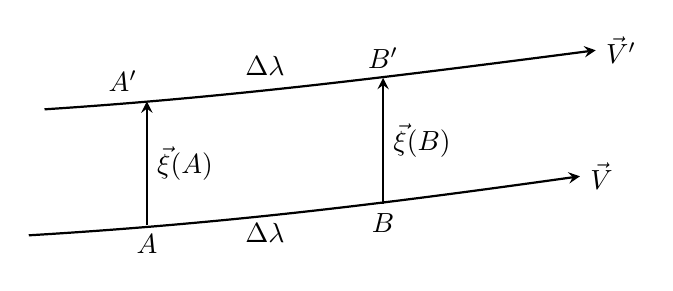
\begin{tikzpicture}[
    >=stealth,                     % lowercase = old arrows library
    curve/.style={thick},
    connector/.style={->,thick}
]

% ---- lower curve (carries V) ----
\draw[curve,->]
    (-0.5,0)
    .. controls (2,0.15) and (4,0.4) .. (6.5,0.75)
    node[right] {$\vec V$};

% ---- upper curve (carries V') ----
\draw[curve,->]
    (-0.3,1.6)
    .. controls (2,1.75) and (4,2.0) .. (6.7,2.35)
    node[right] {$\vec V'$};

% ---- points ----
\coordinate (A)  at (1,0.13);
\coordinate (B)  at (4,0.4);
\coordinate (Ap) at (1,1.7);
\coordinate (Bp) at (4,2.0);

% ---- connecting (deviation) vectors ----
\draw[connector] (A) -- (Ap) node[midway,right] {$\vec\xi(A)$};
\draw[connector] (B) -- (Bp) node[midway,right] {$\vec\xi(B)$};

% ---- labels ----
\node[below] at (A)  {$A$};
\node[below] at (B)  {$B$};
\node[above left] at (Ap) {$A'$};
\node[above] at (Bp) {$B'$};
\node[below] at (2.5,0.28) {$\Delta\lambda$};
\node[above] at (2.5,1.9)  {$\Delta\lambda$};
\end{tikzpicture}
\end{center}

If we have two nearby geodesics parameterized by an affine parameter $\lambda=x^0$ (choosing the local inertial frame for point $A$ which gives $V=\delta^\alpha_0$ and $V'=\delta^\alpha_0$), and let $\vec V$ and $\vec V'$ be the tangent vectors to the geodesics. We have the geodesic equation:
\begin{equation}
    \frac{d^2x^\alpha}{d\lambda^2}\Big|_A=0
\end{equation}

Then, at point $A'$, we have the geodesic equation:
\begin{equation}
    \frac{d^2x'^\alpha}{d\lambda^2}\Big|_{A'}+\Gamma^\alpha_{00}=0
\end{equation}

We can also write down
\begin{equation}
    \Gamma^\alpha _{00}\cong \Gamma^\alpha_{00,\beta}\xi^\beta
\end{equation}
Then we will have
\begin{equation}
    \frac{d^2x^\alpha}{d\lambda^2}\Big|_{A'}=-\Gamma^\alpha_{00,\beta}\xi^\beta
\end{equation}

From this, we can compute the change in the seperaction vector $\xi$
\begin{equation}
    \frac{d^2\xi^\alpha}{d\lambda^2}=\frac{d^2x^\alpha}{d\lambda^2}\Big|_{A'}-\cancelto{0}{\frac{d^2x^\alpha}{d\lambda^2}\Big|_A}=-\Gamma^\alpha_{00,\beta}\xi^\beta
\end{equation}

With this, if we consider the Riemann curvature tensor, we can write down the geodesic deviation equation by considering the second covariant derivative (Directional Derivative along $\lambda$) of the separation vector $\xi^\alpha$ along the geodesic:
\begin{equation}
    \begin{split}
\frac{D^2 \xi^\alpha}{D \lambda^2} &= \nabla_V(\nabla_V \xi^\alpha)\\
&=\frac{d}{d\lambda}\left(\nabla_V \xi^\alpha \right)+\Gamma^\alpha_{\beta 0}(\nabla_V \xi^\beta)\\
&=\frac{d^2\xi^\alpha}{d\lambda^2}+\Gamma^\alpha_{\beta 0,0}\xi^\beta+\cancelto{0}{\Gamma^\alpha_{\beta0}\frac{d\xi}{d\lambda}}\\
&=(\Gamma^\alpha_{0\beta,0}-\Gamma^\alpha_{00,\beta})\xi^\beta=\Ric^\alpha_{00\beta}\xi^\beta\\
&=\Ric^\alpha_{\beta\gamma\delta} V^\beta V^\gamma \xi^\delta\\
    \end{split}
\end{equation}
\subsection{Ricci Tensor and Scalar Curvature}
The Ricci tensor is obtained by contracting the Riemann curvature tensor:
\begin{equation}
R_{\mu\nu} = R^\lambda_{\mu\lambda\nu}
\end{equation}
in which it represents the trace of the Riemann curvature tensor and encodes information about the curvature of the manifold in a more compact form. The Ricci tensor is symmetric, meaning that we also have $R_{\mu\nu} = R_{\nu\mu}$.

If we then contract the Ricci tensor, we obtain the scalar curvature $R$:
\begin{equation}
R = g^{\mu\nu} R_{\mu\nu}
\end{equation}
The scalar curvature is a single number that describes the overall curvature of the manifold at a point.

\subsection{Bianchi Identities and the Einstein Tensor}
We have the Bianchi identities, which are a set of differential identities satisfied by the Riemann curvature tensor. They can be expressed as:
\begin{equation}
\nabla_\lambda \Ric^\rho_{\sigma\mu\nu} + \nabla_\mu \Ric^\rho_{\sigma\nu\lambda} + \nabla_\nu \Ric^\rho_{\sigma\lambda\mu} = 0
\end{equation}

We first lower the index of the Riemann curvature tensor to obtain:
\begin{equation}
\nabla_\lambda \Ric_{\rho\sigma\mu\nu} + \nabla_\mu \Ric_{\rho\sigma\nu\lambda} + \nabla_\nu \Ric_{\rho\sigma\lambda\mu} = 0
\end{equation}

And then we can contract the indices $\rho$ and $\mu$ to obtain:
\begin{equation}
    \nabla_\lambda\Ric_{\sigma\nu}+\nabla_\mu\Ric^\mu_{\sigma\nu\lambda}-\nabla_\nu\Ric_{\sigma\lambda}=0
\end{equation}

Contracting it on $\sigma$ and $\nu$ again with $g^{\sigma\nu}$ (note that the second term contracts slots 2 and 3 of the Riemann tensor rather than the canonical slots 1 and 3, so applying the first-pair antisymmetry $R_{\alpha\sigma\nu\lambda}=-R_{\sigma\alpha\nu\lambda}$ to bring it to Ricci form generates a minus sign; the third term requires only a dummy relabel $\sigma\to\mu$, which is sign-free), we have:
\begin{equation}
    \nabla_\lambda \Ric -\nabla_\mu\Ric^\mu{}_\lambda-\nabla_\mu\Ric^\mu{}_\lambda=\nabla_\lambda \Ric -2\nabla_\mu\Ric^\mu{}_\lambda=0
\end{equation}
We can define the Einstein tensor $G_{\mu\nu}$ as a combination of the Ricci tensor and the scalar curvature:
\begin{equation}
G_{\mu\nu} = \Ric_{\mu\nu} - \frac{1}{2} \Ric g_{\mu\nu}
\end{equation}

In which if we take the covariant derivative of the Einstein tensor, we have:
\begin{equation}
\nabla^\mu G_{\mu\nu} = 0
\end{equation}

\subsection{In Weak Gravitational Field}

In a slightly curved spacetime, we have the metric tensor given by:
\begin{equation}
    ds^2=-(1+2\phi)dt^2+(1-2\phi)(dx^2+dy^2+dz^2)
\end{equation}

Lets now consider a freely falling particle in this spacetime. The four velocity of the particle $U^mu$ must satisfy the geodesic equation:
\begin{equation}
    \nabla_U U^\mu = 0
\end{equation}

Note that all the multiple of the proper time is also an affine parameter, so the four momentum $P^\mu$ must also satisfy the geodesic equation:
\begin{equation}
    \nabla_P P^\mu = 0
\end{equation}

This euqation can also be used for photon but not the one for four velocity since $m=0$.

If the particle has non relativistic speed, we can write down the geodesic equation as:
\begin{equation}
    m\frac{dP^0}{d\tau}+\Gamma^0_{\alpha\beta}P^\alpha P^\beta=0
\end{equation} 
by considering the fact that $P^0>>P^1$ and $P^0\approx m$. Then we have:
\begin{equation}
    \Gamma^0_{\alpha\beta}P^\alpha P^\beta\approx \Gamma^0_{00}P^0 P^0\approx \Gamma^0_{00}m^2
\end{equation}
Then we have:
\begin{equation}
    \frac{dP^0}{d\tau}=-\Gamma^0_{00}m
\end{equation}

To compute $\Gamma^0_{00}$, we have:
\begin{equation}
    \Gamma^0_{00}=\frac{1}{2}g^{0\alpha}( g_{0\alpha,0}+ g_{0\alpha,0}- g_{00,\alpha})
\end{equation}

As the metric is diagonal, thus $g^{0\alpha}$ in nonzero only when $\alpha=0$. Then we have:
\begin{equation}
    \Gamma^0_{00}=\frac{1}{2}g^{00} g_{00,0}=\frac{1}{2}\frac{1}{-(1+2\phi)}(-2 \phi_{,0})\approx \phi_{,0}
\end{equation}
The last term comes from the taylor expansion of the fraction and taking the lowest order term.

Also, we have that $P^0\approx m$, thus we have:
\begin{equation}
    \frac{dP^0}{d\tau}=-m \phi_{,0}
\end{equation}

The spatial component of the geodesic also gives us the Newton's second law:
\begin{equation}
  m\frac{dP^i}{d\tau}+\Gamma^i_{00}(P^0)^2=0
\end{equation}
Then
\begin{equation}
    m\frac{dP^i}{d\tau}=-\Gamma^i_{00}(P^0)^2
\end{equation}

While we compute the Christoffel symbol:
\begin{equation}
    \Gamma^i_{00}=\frac{1}{2}g^{i\mu} g_{\mu0,0}+g_{\mu0,0}-g_{00,\mu}
\end{equation}

Under the metric, we have:
\begin{equation}
    g^{i\mu}=(1-2\phi)^{-1}\delta^{i\mu}
\end{equation}
Then we have:
\begin{equation}
    \Gamma^i_{00}=\frac{1}{2}(1-2\phi)^{-1}\delta^{i\mu}(g_{\mu0,0}+g_{\mu0,0}-g_{00,\mu})
\end{equation}
We have $\mu$ going from 1 to 3 as $\delta^{i0}=0$ and basically $g_{\mu0,0}=0$. So we have
\begin{equation}
    \begin{split}
    \Gamma^i_{00}&=-\frac{1}{2}g_{00,\mu}\delta^{i\mu}\\
    &=\frac{1}{2}(2\phi)_{,\mu}\delta^{ij}
    \end{split}
\end{equation}

Then we can conclude that
\begin{equation}
    \frac{dP^i}{d\tau}=-m\phi_{,i}
\end{equation}

Which is basically equivalent to
\begin{equation}
    \frac{dP}{dt}=-m\nabla\phi
\end{equation}

\subsection{Conserved Quantity}
The claim is, if the metric is independent of some coordinate $x^i$, then the corresponding momentum is conserved. From Newton's perspective, gravity is a force, extra energy is provided. But there is an exception:

If we write out the geodesic
\begin{equation}
    p^\alpha p_{\beta;\alpha}=0
\end{equation}
or
\begin{equation}
    \frac{dp_\beta}{d\lambda}-\Gamma^\alpha_{\beta\gamma}p_\alpha p^\gamma=0
\end{equation}
Then we have,
\begin{equation}
    m\frac{dp_\beta}{d\tau}=\Gamma^\gamma_{\beta\alpha}p^\alpha p_\gamma
\end{equation}

Then we try to compute the christoffel symbol:
\begin{equation}
    \begin{split}
    \Gamma^\gamma_{\alpha\beta}p^\alpha p_\gamma &= \frac{1}{2}g^{\gamma\mu}\left(g_{\mu\alpha,\beta}+g_{\mu\beta,\alpha}-g_{\alpha\beta,\mu}\right)p^\alpha p_\gamma\\
    &= \frac{1}{2}\left(g_{\mu\alpha,\beta}+g_{\mu\beta,\alpha}-g_{\alpha\beta,\mu}\right)p^\alpha p^\mu\\
    \end{split}
\end{equation}

Note that $g_{\mu\beta,\alpha}-g_{\alpha\beta,\mu}$ is antisymmetric while $p^\alpha p^\mu$ is symmetric, thus we have the product to be zero. Then we have:
\begin{equation}
    \Gamma^\gamma_{\alpha\beta}p^\alpha p_\gamma = \frac{1}{2}g_{\mu\alpha,\beta}p^\alpha p^\mu
\end{equation}

Then we can conclude that
\begin{equation}
    \boxed{m\frac{dp_\beta}{d\tau}=\frac{1}{2}g_{\alpha\mu,\beta}p^\alpha p^\mu}
\end{equation}

We can tell that, if $g_\alpha\nu$ is independent of some coordinate $x^\beta$, then the component $p_\beta$ is conserved along the geodesic. This is a manifestation of Noether's theorem, which states that symmetries in the spacetime metric lead to conserved quantities along geodesics.

\section{Stress Energy Tensor of Dust}
For perfect fluids, the stress-energy tensor is given by:
\begin{equation}
T^{\mu\nu} = (\rho + p) u^\mu u^\nu + p g^{\mu\nu}
\end{equation}
While the component of the stress-energy tensor means the energy density, the pressure, and the momentum flux of the matter distribution. The stress-energy tensor is a symmetric rank-2 tensor that describes the distribution of energy and momentum in spacetime which gives
\begin{equation}
    T_{\mu\nu}=T_{\nu\mu}
\end{equation}

It serves as the source term in Einstein's field equations, which relate the curvature of spacetime to the energy and momentum content.

For some special cases, we can have the conservation of the stress-energy tensor, which is expressed mathematically as:
\begin{equation}
\nabla_\mu T^{\mu\nu} = 0
\end{equation}


\section{Einstein's Field Equations}

In Newtonian theory, mass density is the source of gravity. In General Relativity, we want something similar while giving an invariant theory. Then one important quantity we want to consider is the energy-stress tensor $T$. Thus we have
\begin{equation}
    O(g)=kT
\end{equation}

From the Newtonian Theory, we know that, $O$ must be a second order differential operator that produce a tensor of rank (2,0) and be a combination of $g_{\mu\nu,\lambda\sigma}$, $g_{\mu\nu,\lambda}$ and $g_{\mu\nu}$

The quantity that satisfy the condition is the Ricci Tensor and the Scalar Curvature. In fact, any tensor in the following form satisfy the condition:
\begin{equation}
    O^{\alpha\beta}= \Ric^{\alpha\beta}+\mu g^{\alpha\beta}\Ric + \Lambda g^{\alpha\beta}
\end{equation}

For some constant $\mu$ and $\Lambda$. To find $\mu$, we use the condition
\begin{equation}
    \boxed{T^{\alpha\beta}_{~~~;\beta}=0}
\end{equation}

Then we have

\begin{equation}
    O^{\alpha\beta}_{~~~;\beta}=\Ric^{\alpha\beta}_{~~~;\beta}+\mu g^{\alpha\beta}\Ric_{;\beta}=0
\end{equation}

Then by the definition of the Einstein Tensor, we have $\mu=-1/2$. Then we arrive the expression of the Einstein Field Equation

\begin{equation}
    G^{\alpha\beta}+\Lambda g^{\alpha\beta}=kT^{\alpha\beta}
\end{equation}

If we pick $\Lambda=0$, and using the result from Netonian lmit, we have $k=8\pi G$. Then we have the Einstein Field Equation in the form of
\begin{equation}
    G^{\alpha\beta}=8\pi T^{\alpha\beta}
\end{equation}

\subsection{Lorentz Transformation and Gauge Transformation}

In the weak gravitational field, we have nearly lorentzian metric. Then we can write down the metric as
\begin{equation}
    g_{\mu\nu}=\eta_{\mu\nu}+h_{\mu\nu} ~~~|h_{\mu\nu}|\ll 1
    \label{eq:weak-field}
\end{equation}

In SR, we have the Lorentz transformation as
\begin{equation}
    \Lambda = \begin{pmatrix}
\gamma & -\beta\gamma & 0 & 0 \\
-\beta\gamma & \gamma & 0 & 0 \\
0 & 0 & 1 & 0 \\
0 & 0 & 0 & 1
\end{pmatrix}
\end{equation}

Then we have 
\begin{equation}
    g_{\bar{\alpha}\bar{\beta}}=\Lambda^\mu_{\bar{\alpha}}\Lambda^\nu_{\bar{\beta}} \eta_{\mu\nu} + \Lambda^\mu_{\bar{\alpha}} \Lambda^\nu_{\bar{\beta}} h_{\mu\nu}
\end{equation}

Leads to

\begin{equation}
    g_{\bar{\alpha}\bar{\beta}} = \eta_{\bar{\alpha}\bar{\beta}}+h_{\bar{\alpha}\bar{\beta}}
\end{equation}

With the definition
\begin{equation}
    \boxed{h_{\bar{\alpha}\bar{\beta}}:=\Lambda^\mu_{\bar{\alpha}}\Lambda^\nu_{\bar{\beta}}h_{\mu\nu}}
\end{equation}

Note that this is then just a space-time with flat and a tensor $h_{\mu\nu}$. Then we know that all the physical field can be defined in terms of $h_{\mu\nu}$.

We move on the gauge transformation, which is a small change on the coordinate system that keeps Eq.\ref{eq:weak-field} to be true. Then we have the transformation as

\begin{equation}
    x^{\bar{\alpha}}=x^\alpha+\xi^\alpha ~~~|\xi^\alpha|\ll 1
\end{equation}

Then we have the metric transformation as
\begin{equation}
    \Lambda^{\bar{\alpha}}_\mu=\frac{\partial x^{\bar{\alpha}}}{\partial x^\mu}=\delta^{\bar{\alpha}}_\mu+\xi^{\bar{\alpha}}_{,\mu}
\end{equation}

and

\begin{equation}
    \Lambda^\alpha_{\bar\beta} = \delta^\alpha_\beta - \xi^\alpha_{,\beta} + O(|\xi^\alpha_{,\beta}|^2)
\end{equation}

Where the later term is from the chain rule of differentiation.

Then to the first order, we have 
\begin{equation}
    g_{\alpha'\beta'}=\eta_{\alpha\beta}+h_{\alpha\beta}-\xi_{\alpha,\beta}-\xi_{\beta,\alpha}
\end{equation}

Then we have the change in $h_{\alpha\beta}$ as

\begin{equation}
    \boxed{h_{\alpha'\beta'}=h_{\alpha\beta}-\xi_{\alpha,\beta}-\xi_{\beta,\alpha}}
\end{equation}
If $\xi$ is small then $h_{\mu\nu}$ is still small. We can also show that to the first order, we can express the covariant curvature tensor as 
\begin{equation}
    \boxed{\Ric_{\alpha\beta\mu\nu}=\frac{1}{2}(h_{\alpha\nu,\beta\mu}+h_{\beta\mu,\alpha\nu}-h_{\alpha\mu,\beta\nu}-h_{\beta\nu,\alpha\mu})}
\end{equation}

As the derivative of $\eta_{\mu\nu}$ is zero.

\subsection{Weak-Field Einstein Equation}

For any symmetric $h_{\alpha\beta}$ that is related by Eq. \ref{eq:weak-field} for some $\xi$. We say they will produce the same physical effect. We know define some index-rised quantities:

\begin{equation}
    h^\mu_{~\beta}:=\eta^{\mu\alpha}h_{\alpha\beta}
\end{equation}

\begin{equation}
    h^{\mu\nu}:=\eta^{\nu\beta}h^\mu_{~\beta}
\end{equation}

And the trace
\begin{equation}
    h:=h^\mu_{~\mu}
\end{equation}

Also a 'tensor' called the 'Trace Reverse':
\begin{equation}
    \bar{h}^{\alpha\beta}:=h^{\alpha\beta}-\frac{1}{2}\eta^{\alpha\beta}h
\end{equation}

In which
\begin{equation}
    \bar{h}:=\bar{h}^\mu_{~\mu}=-h
\end{equation}

We can then have the Einstein Tensor
\begin{equation}
    G_{\alpha\beta}=-\frac{1}{2}\left[\bar{h}_{\alpha\beta,\mu}^{~~~~~,\mu}+\eta_{\alpha\beta}\bar{h}_{\mu\nu}^{~~~,\mu\nu}-\bar{h}_{\alpha\mu,\beta}^{~~~~~~,\mu}-\bar{h}_{\beta\mu,\alpha}^{~~~~~~,\mu}+\mathcal{O}(h^2)\right]
\end{equation}

We can set $\bar{h}^{\mu\nu}_{~~~,\nu}=0$ by choosing the Lorentz Gauge. Suppose we have $\bar{h}^{\text{old}}_{\mu\nu}$ which the divergence is non zero. Then we have
\begin{equation}
    \bar{h}^{\text{new}}_{\mu\nu}=\bar{h}^{\text{old}}_{\mu\nu}-\xi_{\mu,\nu}-\xi_{\nu,\mu}+\eta_{\mu\nu}\xi^\alpha_{~,\alpha}
\end{equation}

The divergence of the new $\bar{h}$ is
\begin{equation}
    \bar{h}^{\text{(new)},\nu}_{\mu\nu}=\bar{h}^{\text{(old)},\nu}_{\mu\nu}-\Box\xi_\mu
\end{equation}

Where $\Box = \left(-\frac{\partial^2}{\partial t^2}+\nabla^2\right)$ is the d'Alembertian operator or wave operator. If the divergence of the new $\bar{h}$ is zero, then we have
\begin{equation}
    \Box\xi_\mu=\bar{h}^{\text{(old)},\nu}_{\mu\nu}
\end{equation}

Since the choice of $\xi$ is arbitrary, we can always find a solution to the above equation. Then we have the Einstein Tensor in the Lorentz Gauge as
\begin{equation}
    G_{\alpha\beta}=\frac{1}{2}\left[\bar{h}_{\alpha\beta,\mu}^{~~~~~,\mu}+\mathcal{O}(h^2)\right]=-\frac{1}{2}\Box\bar{h}_{\alpha\beta}
\end{equation}

Which then we have the Einstein Field Equation in the weak field as
\begin{equation}
    \Box\bar{h}_{\alpha\beta}=-16\pi T_{\alpha\beta}
\end{equation}

And this is the quation for linearized gravity.
\section{Gravitational Wave}

We take the wave operator in vaccum condition, which means $T_{\alpha\beta}=0$. Then we have
\begin{equation}
    \Box\bar{h}_{\alpha\beta}=0
\end{equation}

For this particular case, we can have the complex solution as
\begin{equation}
    \bar{h}_{\alpha\beta}=A_{\alpha\beta}e^{ik_\mu x^\mu}
\end{equation}

with $A_{\alpha\beta}$ as the complex polarization tensor. The physical field is the real part of the solution.

Plug it back to the wave equation, we have
\begin{equation}
    \Box e^{ikx} = (ikx_\alpha)(ik^\alpha)e^{ikx} = -k_\alpha k^\alpha e^{ikx}
\end{equation}

For the non trivial $A_{\mu\nu}\neq 0$ we must have $k_\alpha k^\alpha=0$. Then we have the wave vector $k^\mu$ is null. This means that the gravitational wave propagates at the speed of light.

Now we want to look at the constraint on $A_{\mu\nu}$. We have the Lorentz Gauge condition as
\begin{equation}
    \bar{h}^{\mu\nu}_{~~~,\nu}=0
\end{equation}
Which gives us the Transversality condition on the polarization tensor:
\begin{equation}
    k_\nu A^{\mu\nu}=0
\end{equation}

For the plane wave solution, we can have 4 extra gauge freedom from the harmonic solution properties (does not break the Lorentz Gauge condition). We can use this freedom to set the trace of $A_{\mu\nu}$ to zero, which is known as the traceless condition:
\begin{equation}
    A^\mu_{~\mu}=0
\end{equation}

While $A_{\mu\nu}$ is symmetric, we have 10 independent components. The Lorentz gauge and the TT gauge conditions reduce the number of independent components to 2. These two independent components correspond to the two polarization states of gravitational waves, often denoted as $+$ and $\times$ polarizations. We have the form for the polarization tensor as
\begin{equation}
    A_{\mu\nu} = \begin{pmatrix}
0 & 0 & 0 & 0 \\
0 & A_+ & A_\times & 0 \\
0 & A_\times & -A_+ & 0 \\
0 & 0 & 0 & 0
\end{pmatrix}
\end{equation}

\subsection{Effect on particle by the wave}

For a free particle that is free falling, it follows the geodesic:
\begin{equation}
    \frac{d}{d\tau}U^\alpha+\Gamma^\alpha_{~\mu\nu} U^\mu U^\nu = 0
\end{equation}

We should investigate the acceleration of the particle. Assuming it is initially at rest, in flat spacetime. Then undergo the perturbation of a gravitational wave. We have:

\begin{equation}
    \left(\frac{d U^\alpha}{d \tau}\right)_0 =  -\Gamma ^\alpha _{~00} = -\frac{1}{2}{ \eta^{\alpha\beta}}(h_{0\beta,0}+h_{\beta0,0}-h_{00,\beta})
\end{equation}

By the TT gauge, we can choose
\section{Black Holes and Singularities}
\subsection{Schwarzchild's Solution}
\subsection{Kerr's Solution}

\section{Thermodynamics in Black Hole}

\subsection{Area Theorem}

\subsection{Holographic Principle}

\section{Cosmology}




\section{Conformal Transformations in General Relativity}

\section{Penrose Diagrams}

\section{Gravitational Lensing}

\section{Self Force}

\end{document}
